% Drop-in Section II proposal. Original manuscript and experiment code untouched.
% Requires the original paper macros/packages plus tikz for figure1_interface.tex.
% Remove the old fig:scale environment before inserting this section.
\section{Simulation Models, Attitude Baseline, and Actuator Interface}
\label{sec:problem}
\subsection{MuJoCo Platforms and CF2 Actuation Extension}
We use Crazyflie 2.0 (CF2) and Skydio X2 models derived from MuJoCo
Menagerie \cite{menagerieModels}. Each vehicle has six rigid-body degrees of freedom: three
translations and three rotations, represented by seven free-joint position
coordinates (position and unit quaternion) and six velocity coordinates.
The attitude controller requests three body torques; a separate classical
height loop requests collective thrust. Thus attitude tracking is evaluated
in a freely translating model, not an attitude-only joint model.

The upstream CF2 interface provides collective thrust and three abstract
body-moment channels; its documentation identifies the original actuator
limits as arbitrary and requiring tuning \cite{menagerieCF2}. Our four-rotor actuation extension replaces that
interface with four nonnegative, spatially located thrust inputs while
retaining the source mass, inertia, and visual geometry. Rotor moment arms
and signed reaction-torque coefficients define an explicit allocation
matrix, making the coupling between collective thrust, attitude torque,
and individual actuator limits testable. This is a model-interface
contribution, not a complete aerodynamic identification of CF2.

\begin{table}[!ht]
\centering
\caption{Compiled simulation-model characteristics. CF2 authority is
scaled relative to the upstream model limit, not a manufacturer rating.
Hardware comparisons are given in Table~\ref{tab:manufacturer}.}
\label{tab:models}
\setlength{\tabcolsep}{3pt}
\footnotesize
\begin{tabular}{@{}p{0.40\linewidth}p{0.27\linewidth}p{0.25\linewidth}@{}}
\toprule
Property & CF2 rotor model & X2 model\\
\midrule
Mass $M$ (kg) & $0.027$ & $1.325$\\
Rotor $|p_x|,|p_y|$ (m) & $0.0325,0.0325$ & $0.14,0.18$\\
Reaction magnitude $|\kappa_i|$ (m) & $0.005$ & $0.0201$\\
Unscaled rotor limit (N) & $0.0875$ & $13$\\
Main-test authority scale & $1.5$ & $1$\\
Main-test rotor limit (N) & $0.13125$ & $13$\\
Main-test total limit (N) & $0.525$ & $52$\\
Maximum thrust/weight & $1.321\to1.982$ & $4.001$\\
Rigid-body integrator & RK4 & Euler\\
Experiment timestep (s) & $0.0005$ & $0.0005$\\
Motor activation/RPM states & None & None\\
\bottomrule
\end{tabular}
\end{table}

For CF2, the unscaled model's total thrust limit is $0.35$ N. We evaluate
a rotor-interface model with increased actuator authority: multiplying
$f_{\max,i}$ by $1.5$ yields $0.525$ N total
(Table~\ref{tab:models}). This raises the modeled maximum thrust/weight
from $1.321$ to $1.982$ at $g=9.81$ m/s$^2$. For physical perspective,
constant-height flight at a single-axis $45^\circ$ tilt requires
$T/(Mg)=1/\cos45^\circ=\sqrt{2}$ even before reserving differential-thrust
margin. The unscaled model cannot meet that idealized requirement; this
does not establish such a limitation for stock CF2 hardware. The scale
changes a simulation thrust bound, not rotor speed, stock propulsion
capability, or tracking performance by $50\%$. Mass, inertia, and reaction
coefficients are unchanged. PD and CMG use the same model and actuator
bounds; any benefit from increased model authority is therefore distinct
from the benefit of neural augmentation.

\begin{table}[!ht]
\centering
\caption{Simulation parameters versus manufacturer information.
``Not reported'' refers to the manufacturer sources reviewed, not proof
that the parameter is unavailable elsewhere.}
\label{tab:manufacturer}
\setlength{\tabcolsep}{3pt}
\footnotesize
\begin{tabular}{@{}>{\raggedright\arraybackslash}p{0.25\linewidth}>{\raggedright\arraybackslash}p{0.30\linewidth}>{\raggedright\arraybackslash}p{0.37\linewidth}@{}}
\toprule
Quantity & Simulation & Manufacturer information\\
\midrule
CF2 mass & $27$ g & $27$ g \cite{bitcrazeCF20Specs}\\
X2 mass & $1325$ g & $1325$ g with battery \cite{skydioX2ESpecs}\\
CF2 total thrust & $0.350\to0.525$ N & $0.568$ N measured at $93.75\%$ PWM\textsuperscript{a} \cite{bitcrazeThrustMeasurements}\\
X2 rotor limit & $13$ N per rotor & Not reported \cite{skydioX2ESpecs}\\
CF2 motor response & No motor dynamics & $\sim180$ ms: $0\to25{,}000$ RPM\textsuperscript{b} \cite{bitcrazeMotorResponse}\\
Inertia tensors & CF2 inherited; X2 geometry-derived & Not reported in product specifications \cite{bitcrazeCF20Specs,skydioX2ESpecs}\\
\bottomrule
\end{tabular}
\par\smallskip
\begin{minipage}{0.97\linewidth}
\scriptsize
\textsuperscript{a}Historical total-thrust measurement with a power-supply
test setup, not a guaranteed continuous battery-powered rating.
\textsuperscript{b}One motor's reported full-command response with a
charged battery; not an identified first-order time constant.
\end{minipage}
\end{table}

The masses agree with published specifications, but this does not
validate all dynamic parameters (Table~\ref{tab:manufacturer}). Bitcraze's
historical measurement of $57.9$ gram-force corresponds to approximately
$0.568$ N; the evaluated $0.525$ N limit is about $7.5\%$ below that
operating point \cite{bitcrazeThrustMeasurements}. This supports a plausible
thrust scale, not hardware validation, and does not establish that a
stronger-than-stock motor is required. CF2 inertia is inherited from
Menagerie, which cites system-identification work \cite{menagerieCF2}; the
rotor-extension moment arms and $|\kappa_i|=0.005$ m remain design
assumptions. X2 inertia, $13$ N rotor limits, and $|\kappa_i|=0.0201$ m are
simulation parameters, not confirmed manufacturer characteristics.

Geometric dimensions also require like-for-like definitions. Bitcraze
lists $92\times92\times29$ mm motor-to-motor/height dimensions
\cite{bitcrazeCF20Specs}; our sites give an opposite-motor separation of
$91.92$ mm. Skydio lists an unfolded flying envelope of approximately
$663\times569\times211$ mm \cite{skydioX2ESpecs}, whereas the model's rotor
centers span $280\times360$ mm. Center spacing and overall flying envelope
are different quantities and do not by themselves establish geometric
agreement or mismatch. Propulsion identification, motor and battery
dynamics, and experimental validation remain necessary for hardware
transfer; no endurance or electrical-power fidelity is claimed.

MuJoCo \cite{todorov2012mujoco} integrates rigid-body motion, gravity, site-applied actuator
wrenches, and enabled passive/contact forces. Both models specify air
density $1.225$ kg/m$^3$ and viscosity $1.8\times10^{-5}$ Pa\,s; their
default inertia-based fluid model \cite{mujocoFluid} is a coarse drag approximation, not
rotor-resolved aerodynamics. The runner overrides the timestep but retains
each model's integrator. Actuators apply algebraic thrust commands without
motor activation dynamics. Although gyro, accelerometer, and orientation
sensors are defined, the evaluated feedback is read directly from
\texttt{qpos}/\texttt{qvel}; optional measurement perturbations are separate
runner settings. These experiments do not establish performance with a
hardware state estimator.

%% Editable, code-aligned replacement for fig:scale. Requires tikz.
\begin{figure}[t]
\centering
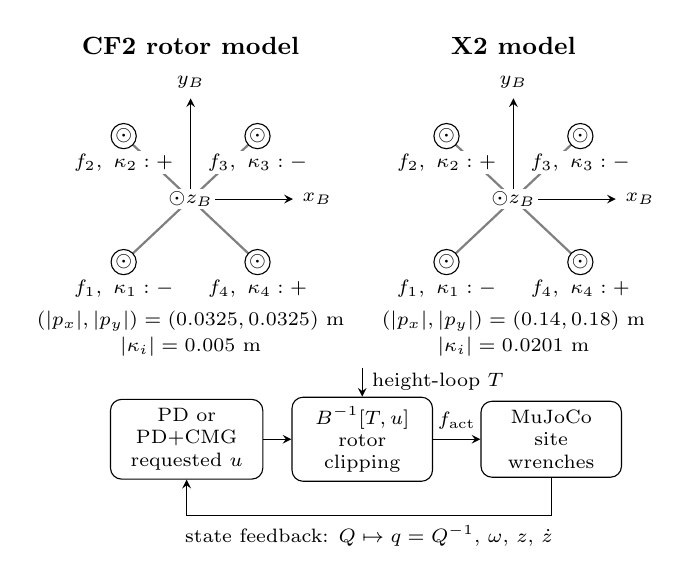
\begin{tikzpicture}[x=1cm,y=1cm,font=\scriptsize,>=stealth]
\foreach \off/\title/\dims/\kap in {0/CF2 rotor model/{0.0325, 0.0325}/0.005,4.1/X2 model/{0.14, 0.18}/0.0201}{
 \begin{scope}[shift={(\off,0)}]
 \node[font=\small\bfseries] at (0,1.95) {\title};
 \draw[gray,thick] (-.85,-.8)--(.85,.8) (-.85,.8)--(.85,-.8);
 \draw[->] (0,0)--(1.3,0) node[right] {$x_B$};
 \draw[->] (0,0)--(0,1.28) node[above] {$y_B$};
 \node[fill=white,inner sep=1pt] at (0,0) {$\odot z_B$};
 \foreach \xx/\yy/\id/\sgn in {-.85/-.8/1/-, -.85/.8/2/+, .85/.8/3/-, .85/-.8/4/+}{
  \draw[fill=white] (\xx,\yy) circle (.16);
  \node at (\xx,\yy) {$\odot$};
  \node[fill=white,inner sep=1pt] at (\xx,\yy-.34) {$f_{\id},\ \kappa_{\id}:\sgn$};
 }
 \node at (0,-1.55) {$(|p_x|,|p_y|)=(\dims)$ m};
 \node at (0,-1.88) {$|\kappa_i|=\kap$ m};
 \end{scope}
}
\node[draw,rounded corners,align=center,text width=1.7cm,minimum height=.75cm] (ctrl) at (-.05,-3.05) {PD or PD+CMG\\requested $\bm u$};
\node[draw,rounded corners,align=center,text width=1.55cm,minimum height=.75cm] (mix) at (2.18,-3.05) {$B^{-1}[T,\bm u\T]\T$\\rotor clipping};
\node[draw,rounded corners,align=center,text width=1.55cm,minimum height=.75cm] (plant) at (4.58,-3.05) {MuJoCo\\site wrenches};
\draw[->] (ctrl)--(mix);
\draw[->] (mix)--node[above] {$\bm f_{\rm act}$}(plant);
\draw[->] (2.18,-2.14)--node[right] {height-loop $T$}(mix.north);
\draw[->] (plant.south)--(4.58,-4.02)--node[below,align=center] {state feedback: $Q\mapsto q=Q^{-1}$, $\bm\omega$, $z$, $\dot z$}(-.05,-4.02)--(ctrl.south);
\end{tikzpicture}
\caption{Code-aligned actuation and feedback interface. Top: body-axis
projections, drawn at independent scales, with rotor numbering matching
the mixer columns. Circles with dots indicate $+z_B$ thrust; $+/-$ labels
give reaction-torque signs, not simulated rotor speeds. X2 site heights
are $0.05$ m for rotors 1--2 and $0.08$ m for 3--4; CF2 sites have zero
height. Bottom: both controllers use the same thrust allocation, clipping,
and state-feedback interface. Table~\ref{tab:models} specifies model authority,
not a manufacturer rating; Table~\ref{tab:manufacturer} provides the hardware comparison.
\eqref{eq:mixer} distinguishes requested from realized wrench.}
\label{fig:scale}
\end{figure}


\subsection{Quaternion Convention and Error}
Let $Q\in\mathbb S^3$ be the scalar-first Hamilton quaternion mapping body
coordinates to inertial coordinates, and let $\bm\omega$ be body angular
velocity. With physical inertia $\bm J\succ0$ about the center of mass,
expressed in body axes, the free-flight rotational balance is
\begin{align}
 \dot Q&=\tfrac12 Q\otimes[0,\bm\omega\T]\T,\\
 \bm J\dot{\bm\omega}&=\bm\tau_{\rm act}+\bm\tau_{\rm p}
       +\bm\tau_{\rm d}-\bm\omega\times(\bm J\bm\omega).
 \label{eq:plant}
\end{align}
Here $\bm\tau_{\rm p}$ denotes modeled passive torque and
$\bm\tau_{\rm d}$ any applied disturbance; the nominal ideal rigid-body
model sets both to zero. Contact, if present, contributes an additional
external wrench. The requested torque and actuator torque are distinct
signals in Fig.~\ref{fig:scale}.

The controller conjugates MuJoCo's orientation and uses the passive
quaternion $q=Q^{-1}$, so
\begin{equation}
 \dot q=-\tfrac12[0,\bm\omega\T]\T\otimes q.
 \label{eq:passive}
\end{equation}
The desired $q_d$ uses the same convention. Define
\begin{align}
 q_e&=q_d\otimes q^{-1}=[q_{e,0},\bm q_{e,v}\T]\T,\\
 \bm e_q&=\sgnp(q_{e,0})\bm q_{e,v},\qquad \sgnp(0)=1,\\
 \theta_q&=2\operatorname{atan2}(\|\bm q_{e,v}\|_2,|q_{e,0}|)
             \in[0,\pi].
 \label{eq:theta}
\end{align}
The reported error $\theta_q$ is the shortest rotation angle, invariant
under $q_e\mapsto-q_e$. Sign selection introduces a discontinuity at
$q_{e,0}=0$; it does not establish robust hybrid global stability
\cite{mayhew2011hybrid}.
For a desired-frame rate $\bm\omega_d$ satisfying the corresponding
passive kinematics, differentiation gives
\begin{align}
 \dot q_e&=\tfrac12q_e\otimes[0,\bm\omega_e\T]\T,\\
 \bm\omega_e&=\bm\omega-R(q_e)\T\bm\omega_d,\qquad
 \dot q_{e,0}=-\tfrac12\bm q_{e,v}\T\bm\omega_e.
 \label{eq:errkin}
\end{align}
This is a kinematic identity, not a convergence result. Reference Euler
triples parameterize $q_d$ in the passive convention, rather than active
body-to-world Euler commands.

\subsection{Physical Inertia and Implemented PD Gains}
MuJoCo stores principal moments $\bm j_{\rm p}$ in its inertial frame
\cite{mujocoInertial}.
If $R_{BI}$ maps that frame into body axes, the physical inertia is
\begin{equation}
 \bm J=R_{BI}\operatorname{diag}(\bm j_{\rm p})R_{BI}\T.
 \label{eq:inertiaframe}
\end{equation}
The evaluated implementation uses a tuning vector
$\bm j_{\rm tune}=\bm j_{\rm p}$ directly, in the returned array order:
\begin{align*}
 \bm j_{\rm tune}^{\rm CF2}&=(2.3951,2.3951,3.2347)\T10^{-5},\\
 \bm j_{\rm tune}^{\rm X2}&=(0.0607113,0.0364684,0.0254117)\T,
\end{align*}
in kg\,m$^2$. CF2's inertial axes coincide with its body axes. For X2
they do not; its physical body-frame tensor is approximately
\begin{equation}
 \bm J_{\rm X2}=\begin{bmatrix}
 0.0366517&0&-0.0021000\\
 0&0.0254117&0\\
 -0.0021000&0&0.0605280
 \end{bmatrix}\ \mathrm{kg\,m^2}.
\end{equation}
Thus the tuning vector must not be identified with
$\operatorname{diag}(\bm J)$ for both vehicles.

The fixed quaternion PD baseline is
\begin{align}
 \bm k_q&=2\bm j_{\rm tune}\odot\bm\omega_n^2,\qquad
 \bm k_\omega=2\zeta\bm j_{\rm tune}\odot\bm\omega_n,\\
 \bm u_0&=\sat_{\bm\ell}
       (-\bm k_q\odot\bm e_q-\bm k_\omega\odot\bm\omega),
 \label{eq:pd}
\end{align}
where $\odot$ denotes componentwise multiplication,
$\bm\omega_n=(4,4,3.5)\T$ rad/s, $\zeta=0.95$, and
$\sat_{\bm\ell}$ clips component $i$ to $[-\ell_i,\ell_i]$.
For these rotor-interface models, the model-policy torque limits are
$\ell_i=\max(j_{{\rm tune},i}a_i,10^{-6}\ \mathrm{N\,m})$,
with $\bm a=(12,12,10)\T$ rad/s$^2$.
These are controller torque bounds, not guaranteed feasible rotor torques.
The law is quaternion feedback \cite{fresk2013quaternion};
$\bm\omega_n$ parameterizes its gains but is not a verified set of
closed-loop natural frequencies for coupled X2 dynamics.
Desired-rate feedforward and gyroscopic cancellation are omitted.
The identical fixed gains are retained for PD and its CMG augmentation.

For perspective only, take a constant reference, scalar proportional
gain $\bm k_q=k_q\bm1$, the ideal plant
($\bm\tau_{\rm p}=\bm\tau_{\rm d}=0$), no saturation or residual, and a
trajectory confined to one smooth sign branch. Then
$V=\frac12\bm\omega\T\bm J\bm\omega+2k_q(1-|q_{e,0}|)$ gives
$\dot V=-\bm\omega\T\operatorname{diag}(\bm k_\omega)\bm\omega$.
This restricted identity does not prove stability of the anisotropic,
saturated, moving-reference experiments.

\subsection{Requested and Realized Wrench}
For rotor positions $\bm p_i$ in body coordinates, parallel $+z$ thrust
axes, and signed reaction coefficients $\kappa_i$, define
\begin{equation}
 B=\begin{bmatrix}
 1&1&1&1\\p_{1,y}&p_{2,y}&p_{3,y}&p_{4,y}\\
 -p_{1,x}&-p_{2,x}&-p_{3,x}&-p_{4,x}\\
 \kappa_1&\kappa_2&\kappa_3&\kappa_4
 \end{bmatrix}.
 \label{eq:allocationmatrix}
\end{equation}
The signs follow $\bm p_i\times[0,0,f_i]\T$ and the actuator's local
reaction torque $\kappa_i f_i$. Both models have zero body-frame
center-of-mass $x,y$ offsets, so the site's $x,y$ coordinates also give
the relevant center-of-mass moment arms. Figure~\ref{fig:scale} fixes the
rotor ordering used by $B$; $\kappa_i$ has units of meters, not angular
velocity. The runner computes
\begin{equation}
 \begin{aligned}
 \bm f_{\rm req}&=B^{-1}[T,\bm u\T]\T,\\
 \bm f_{\rm act}&=\clip_{[\bm0,\bm f_{\max}]}(\bm f_{\rm req}),\\
 [T_{\rm act},\bm\tau_{\rm act}\T]\T&=B\bm f_{\rm act}.
 \end{aligned}
 \label{eq:mixer}
\end{equation}
Here $\bm u=\bm u_0$ for PD; the CMG path in Section~\ref{sec:architecture}
modifies that requested torque before the same allocation and clipping.
Each $f_i$ is a commanded force in newtons, not a rotor-speed command.
Exact wrench realization requires
$B^{-1}[T,\bm u\T]\T\in[\bm0,\bm f_{\max}]$.
A componentwise torque box is not generally contained in this
collective-dependent feasible set. Clipped inverse allocation is used,
not an optimization-based allocator \cite{monteiro2016allocation}.

Collective thrust remains classical, with $z_d=1$ m:
\begin{equation}
 T=\clip_{[0,2.5Mg]}
 \left(\frac{M[g+6(z_d-z)-4\dot z]}{\max(R(Q)_{33},0.35)}\right).
 \label{eq:collective}
\end{equation}
This expression uses the model's $g=9.81$ m/s$^2$. The height loop reads
free-joint height and vertical velocity; the denominator compensates tilt
with a lower guard. Its upper bound does not supersede individual rotor
limits. The CMG path has no direct collective output, but can affect
height through attitude, tilt compensation, and allocation saturation.
The resulting shared plant interface isolates changes in requested
attitude torque while preserving the same physical simulation for both
controllers.
